\documentclass[compress]{beamer}  % Use [compress] for presentation. [handout]
%=========================================================================================
% Beamer settings
%=========================================================================================\
\mode<presentation>
\usetheme{Boadilla} % Beamer Theme
\useoutertheme[subsection=false]{smoothbars}
\useinnertheme{rectangles}
\usecolortheme{orchid} % Beamer Color Theme
\beamertemplatenavigationsymbolsempty  % No navigation bar.
\setbeamertemplate{footline}[page number]  % Show page number.
%=========================================================================================
% Math Packages
%=========================================================================================\
\usepackage{ifpdf}
\usepackage{amsmath}
\usepackage{amsthm}
\usepackage{amsfonts}
\usepackage{amssymb}
\usepackage{dsfont}
\usepackage{bbm}
\usepackage{enumerate}
\usepackage{hyperref}
\usepackage{url,tabularx,array}
\usepackage{pdfsync}
%=========================================================================================
% Figure and Graphics
%=========================================================================================
\usepackage{graphicx}
\usepackage{caption}
\usepackage{subcaption}
\usepackage{epstopdf}
\epstopdfsetup{outdir=./eps2pdf/}   
\graphicspath{{eps/}{png/}}  
%\usepackage{tikz,pgfplots}
%\usetikzlibrary{arrows}
%\pgfplotsset{compat=newest} 
%\pgfplotsset{plot coordinates/math parser=false}
%=========================================================================================
% Syntax Coloring for Matlab code
%=========================================================================================
\usepackage{courier}
\usepackage{color}
\usepackage{listings}
% Matlab listing macros.
%   First we define the Matlab listing style. There are two classoffset
%   beside the basic keywords. The first offset is for command style 
%   code with purple color. The second offset is the emphisized keywords.
%   Feel free to edit or remove them.
%
%   We provide two commands to use the Matlab code listing style.
%
%   The matlabcode environment:
%       \begin{matlabcode}[additional_styles]
%           put your Matlab code here
%       \end{matlabcode}
%
%   The input method:
%       \inputMatlabCode{filename}[additional_style]

\definecolor{dkgreen}{rgb}{0,0.6,0}  % Comment.
\definecolor{purple}{rgb}{0.6,0,0.6} % String.
\lstloadlanguages{Matlab}
\lstdefinestyle{Matlab}  % Define the Matlab listing style.
{
   language=Matlab,
   basicstyle=\ttfamily,
   numbers=none, % {right, left, none}
   numberstyle=\tiny\color{black},
   stepnumber=1,
   numbersep=10pt,
   backgroundcolor=\color{white},
   tabsize=4,
   showspaces=false,
   showstringspaces=false,
   classoffset=0, %=================================================== 
   frame=single,  % Single frame around code
   keywords={break,case,catch,continue,else,elseif,end,for,function,
             global,if,otherwise,persistent,return,switch,try,while},
   keywordstyle=\color{blue},
   commentstyle=\usefont{T1}{pcr}{m}{sl}\color{dkgreen},
   stringstyle=\color{purple},
   classoffset=1, %===================================================
   morekeywords={all,on,off},keywordstyle=\color{purple},
   classoffset=2, %===================================================
   morekeywords={},
   keywordstyle=\color{black}\bfseries,
   classoffset=0  %===================================================
}

\lstnewenvironment{matlabcode}[1][]{\lstset{style=Matlab,#1}}{}
\newcommand{\inputMatlabCode}[2][]
           {\lstinputlisting[style=Matlab,title=\lstname,#1]{#2}} % Defines the Matlab code listing style and commands.
\newcommand{\tttbf}[1]{\texttt{\textbf{#1}}} % Matlab keywords: typewriter+bf.
\definecolor{blockbody}{rgb}{0.914,0.914,0.953}
\setbeamercolor{block body}{bg = blockbody}
\lstnewenvironment{matlabcodebeamer}[1][]{\lstset{style=Matlab,backgroundcolor=\color{blockbody},#1}}{}
%=========================================================================================
% User Defined Macro
%=========================================================================================
%========== Probability ==========%
	% iid: independent identically distributed
\newcommand{\iid}{\textit{i.i.d.}}
	% Expectation
%\newcommand{\E}[1]{\ensuremath{\operatorname{E}\left[\: #1 \:\right]}}
\newcommand{\E}[2][0]{%
  \ifcase#1 
         \operatorname{\mathbf E}       ( #2       ) 
     \or \operatorname{\mathbf E} \bigl ( #2  \bigr)
     \or \operatorname{\mathbf E} \Bigl ( #2  \Bigr) 
     \or \operatorname{\mathbf E} \biggl( #2 \biggr)
     \or \operatorname{\mathbf E} \Biggl( #2 \Biggr) 
  \else 
         \operatorname{\mathbf E} \mathopen{}\left( #2 \mathclose{}\right)
  \fi}
  
	% Conditional Expectation
%\newcommand{\cE}[2]{\ensuremath{\operatorname{E}\left[\: #1 \:\middle\vert\: #2 \:\right]}}
%% Example:
% $$ \cE{X}{Y} \quad  
%   \cE[1]{X}{Y^2} \quad 
%   \cE[2]{X}{\dfrac{Y}{Z}} \quad 
%   \cE[3]{X}{\dfrac{Y}{Z}}\quad 
%   \cE[4]{X}{\dfrac{Y}{Z}}\quad 
%   \cE[5]{X}{\frac{Y^{\int}}{Z}}$$
\newcommand{\cE}[3][0]{%
  \ifcase#1 
         \operatorname{\mathbf E}       ( #2       \mid  #3       ) 
     \or \operatorname{\mathbf E} \bigl ( #2 \bigm \vert #3 \bigr )
     \or \operatorname{\mathbf E} \Bigl ( #2 \Bigm \vert #3 \Bigr ) 
     \or \operatorname{\mathbf E} \biggl( #2 \biggm\vert #3 \biggr)
     \or \operatorname{\mathbf E} \Biggl( #2 \Biggm\vert #3 \Biggr) 
  \else 
     \operatorname{\mathbf E} \mathopen{}\left( #2  \;\middle\vert\; #3 \mathclose{}\right)
  \fi}

	% Variance
\newcommand{\Var}[1]{\textrm{Var}\left[ #1 \right] }
	% Normal Distribution
\newcommand{\N}[2]{\ensuremath{ \mathcal{N}\left( #1, #2 \right) }}
	% Circular-symmetric Complex Normal Distribution
\newcommand{\CN}[2]{\ensuremath{ \mathcal{CN}\left( #1, #2 \right) }}
	% Covariance
\DeclareMathOperator{\cov}{cov}
	% Probability
%\newcommand{\Prob}[1]{\ensuremath{\Pr\!\left[\: #1 \:\right] }}
\newcommand{\Prob}[2][0]{%
  \ifcase#1 
         \operatorname{\Pr}       ( #2       ) 
     \or \operatorname{\Pr} \bigl ( #2  \bigr)
     \or \operatorname{\Pr} \Bigl ( #2  \Bigr) 
     \or \operatorname{\Pr} \biggl( #2 \biggr)
     \or \operatorname{\Pr} \Biggl( #2 \Biggr) 
  \else 
         \operatorname{\Pr} \mathopen{}\left( #2 \mathclose{}\right)
  \fi}
  
	% Conditional Probability
%\newcommand{\cProb}[2]{\ensuremath{\Pr\!\left[\: #1 \:\middle\vert\: #2 \:\right] }}
\newcommand{\cProb}[3][0]{%
  \ifcase#1 
         \operatorname{\Pr}       ( #2       \mid  #3       ) 
     \or \operatorname{\Pr} \bigl ( #2 \bigm \vert #3 \bigr )
     \or \operatorname{\Pr} \Bigl ( #2 \Bigm \vert #3 \Bigr ) 
     \or \operatorname{\Pr} \biggl( #2 \biggm\vert #3 \biggr)
     \or \operatorname{\Pr} \Biggl( #2 \Biggm\vert #3 \Biggr) 
  \else 
     \operatorname{\Pr} \mathopen{}\left( #2  \;\middle\vert\; #3 \mathclose{}\right)
  \fi}
  
	% Event
\newcommand{\event}[1]{\ensuremath{\left\{ #1 \right\} }}
	% Distributed As
\newcommand{\distas}{\ensuremath{\overset{\textit{d}}{=}}}

\newcommand{\pperp}{\perp\!\!\!\perp}
%========== Matrix ==========%
	% Trace Operator
\DeclareMathOperator{\tr}{tr}
	% Norm
%\newcommand{\norm}[1]{\left|\left| #1 \right|\right|}
\newcommand{\norm}[2][0]{%
  \ifcase#1 
         \lVert #2 \rVert 
     \or \bigl\lVert #2 \bigl\rVert
     \or \Bigl\lVert #2 \Bigl\rVert
     \or \biggl\lVert #2 \biggl\rVert
     \or \Biggl\lVert #2 \Biggl\rVert 
  \else 
         \mathopen{}\left\lVert #2 \mathclose{}\right\rVert
  \fi}

\DeclareMathOperator{\sgn}{sgn}
\DeclareMathOperator{\sinc}{sinc}
\DeclareMathOperator{\diag}{diag}
\DeclareMathOperator{\epi}{epi}
\DeclareMathOperator{\Image}{Im}
\DeclareMathOperator{\conv}{conv}  % Convex hull
\newcommand{\one}{\ensuremath{\mathbbm{1}}}  % Indicator function
\DeclareMathOperator{\spn}{span}  % Linear span

%========== Arithmatic ==========%
\newcommand{\e}{\textrm{e}}


%========== Matrix ==============%
\DeclareMathOperator{\vect}{vec}






% Zero Vector
\newcommand{\vzeros}{\ensuremath{\boldsymbol{0}}}
% One Vector
\newcommand{\vones}{\ensuremath{\boldsymbol{1}}}
% English vector
\newcommand{\va}{\ensuremath{\boldsymbol{a}}}
\newcommand{\vb}{\ensuremath{\boldsymbol{b}}}
\newcommand{\vc}{\ensuremath{\boldsymbol{c}}}
\newcommand{\vd}{\ensuremath{\boldsymbol{d}}}
\newcommand{\ve}{\ensuremath{\boldsymbol{e}}}
\newcommand{\vf}{\ensuremath{\boldsymbol{f}}}
\newcommand{\vg}{\ensuremath{\boldsymbol{g}}}
\newcommand{\vh}{\ensuremath{\boldsymbol{h}}}
\newcommand{\vi}{\ensuremath{\boldsymbol{i}}}
\newcommand{\vj}{\ensuremath{\boldsymbol{j}}}
\newcommand{\vk}{\ensuremath{\boldsymbol{k}}}
\newcommand{\vl}{\ensuremath{\boldsymbol{l}}}
\newcommand{\vm}{\ensuremath{\boldsymbol{m}}}
\newcommand{\vn}{\ensuremath{\boldsymbol{n}}}
\newcommand{\vo}{\ensuremath{\boldsymbol{o}}}
\newcommand{\vp}{\ensuremath{\boldsymbol{p}}}
\newcommand{\vq}{\ensuremath{\boldsymbol{q}}}
\newcommand{\vr}{\ensuremath{\boldsymbol{r}}}
\newcommand{\vs}{\ensuremath{\boldsymbol{s}}}
\newcommand{\vt}{\ensuremath{\boldsymbol{t}}}
\newcommand{\vu}{\ensuremath{\boldsymbol{u}}}
\newcommand{\vv}{\ensuremath{\boldsymbol{v}}}
\newcommand{\vw}{\ensuremath{\boldsymbol{w}}}
\newcommand{\vx}{\ensuremath{\boldsymbol{x}}}
\newcommand{\vy}{\ensuremath{\boldsymbol{y}}}
\newcommand{\vz}{\ensuremath{\boldsymbol{z}}}
% Greek vector
\newcommand{\valpha}{\ensuremath{\boldsymbol{\alpha}}}
\newcommand{\vbeta}{\ensuremath{\boldsymbol{\beta}}}
\newcommand{\vgamma}{\ensuremath{\boldsymbol{\gamma}}}
\newcommand{\vdelta}{\ensuremath{\boldsymbol{\delta}}}
\newcommand{\vepsilon}{\ensuremath{\boldsymbol{\epsilon}}}
\newcommand{\vzeta}{\ensuremath{\boldsymbol{\zeta}}}
\newcommand{\veta}{\ensuremath{\boldsymbol{\eta}}}
\newcommand{\vtheta}{\ensuremath{\boldsymbol{\theta}}}
\newcommand{\viota}{\ensuremath{\boldsymbol{\iota}}}
\newcommand{\vkappa}{\ensuremath{\boldsymbol{\kappa}}}
\newcommand{\vlambda}{\ensuremath{\boldsymbol{\lambda}}}
\newcommand{\vmu}{\ensuremath{\boldsymbol{\mu}}}
\newcommand{\vnu}{\ensuremath{\boldsymbol{\nu}}}
\newcommand{\vxi}{\ensuremath{\boldsymbol{\xi}}}
\newcommand{\vomicron}{\ensuremath{\boldsymbol{\omicron}}}
\newcommand{\vpi}{\ensuremath{\boldsymbol{\pi}}}
\newcommand{\vrho}{\ensuremath{\boldsymbol{\rho}}}
\newcommand{\vsigma}{\ensuremath{\boldsymbol{\sigma}}}
\newcommand{\vtau}{\ensuremath{\boldsymbol{\tau}}}
\newcommand{\vupsilon}{\ensuremath{\boldsymbol{\upsilon}}}
\newcommand{\vphi}{\ensuremath{\boldsymbol{\phi}}}
\newcommand{\vchi}{\ensuremath{\boldsymbol{\chi}}}
\newcommand{\vpsi}{\ensuremath{\boldsymbol{\psi}}}
\newcommand{\vomega}{\ensuremath{\boldsymbol{\omega}}}

% Zero Matrix
\newcommand{\mZeros}{\ensuremath{\boldsymbol{O}}}
% English Matrix
\newcommand{\mA}{\ensuremath{\boldsymbol{A}}}
\newcommand{\mB}{\ensuremath{\boldsymbol{B}}}
\newcommand{\mC}{\ensuremath{\boldsymbol{C}}}
\newcommand{\mD}{\ensuremath{\boldsymbol{D}}}
\newcommand{\mE}{\ensuremath{\boldsymbol{E}}}
\newcommand{\mF}{\ensuremath{\boldsymbol{F}}}
\newcommand{\mG}{\ensuremath{\boldsymbol{G}}}
\newcommand{\mH}{\ensuremath{\boldsymbol{H}}}
\newcommand{\mI}{\ensuremath{\boldsymbol{I}}}
\newcommand{\mJ}{\ensuremath{\boldsymbol{J}}}
\newcommand{\mK}{\ensuremath{\boldsymbol{K}}}
\newcommand{\mL}{\ensuremath{\boldsymbol{L}}}
\newcommand{\mM}{\ensuremath{\boldsymbol{M}}}
\newcommand{\mN}{\ensuremath{\boldsymbol{N}}}
\newcommand{\mO}{\ensuremath{\boldsymbol{O}}}
\newcommand{\mP}{\ensuremath{\boldsymbol{P}}}
\newcommand{\mQ}{\ensuremath{\boldsymbol{Q}}}
\newcommand{\mR}{\ensuremath{\boldsymbol{R}}}
\newcommand{\mS}{\ensuremath{\boldsymbol{S}}}
\newcommand{\mT}{\ensuremath{\boldsymbol{T}}}
\newcommand{\mU}{\ensuremath{\boldsymbol{U}}}
\newcommand{\mV}{\ensuremath{\boldsymbol{V}}}
\newcommand{\mW}{\ensuremath{\boldsymbol{W}}}
\newcommand{\mX}{\ensuremath{\boldsymbol{X}}}
\newcommand{\mY}{\ensuremath{\boldsymbol{Y}}}
\newcommand{\mZ}{\ensuremath{\boldsymbol{Z}}}
% Greek matrix
\newcommand{\mAlpha}{\ensuremath{\boldsymbol{\Alpha}}}
\newcommand{\mBeta}{\ensuremath{\boldsymbol{\Beta}}}
\newcommand{\mGamma}{\ensuremath{\boldsymbol{\Gamma}}}
\newcommand{\mDelta}{\ensuremath{\boldsymbol{\Delta}}}
\newcommand{\mEpsilon}{\ensuremath{\boldsymbol{\Epsilon}}}
\newcommand{\mZeta}{\ensuremath{\boldsymbol{\Zeta}}}
\newcommand{\mEta}{\ensuremath{\boldsymbol{\Eta}}}
\newcommand{\mTheta}{\ensuremath{\boldsymbol{\Theta}}}
\newcommand{\mIota}{\ensuremath{\boldsymbol{\Iota}}}
\newcommand{\mKappa}{\ensuremath{\boldsymbol{\Kappa}}}
\newcommand{\mLambda}{\ensuremath{\boldsymbol{\Lambda}}}
\newcommand{\mMu}{\ensuremath{\boldsymbol{\Mu}}}
\newcommand{\mNu}{\ensuremath{\boldsymbol{\Nu}}}
\newcommand{\mXi}{\ensuremath{\boldsymbol{\Xi}}}
\newcommand{\mOmicron}{\ensuremath{\boldsymbol{\Omicron}}}
\newcommand{\mPi}{\ensuremath{\boldsymbol{\Pi}}}
\newcommand{\mRho}{\ensuremath{\boldsymbol{\Rho}}}
\newcommand{\mSigma}{\ensuremath{\boldsymbol{\Sigma}}}
\newcommand{\mTau}{\ensuremath{\boldsymbol{\Tau}}}
\newcommand{\mUpsilon}{\ensuremath{\boldsymbol{\Upsilon}}}
\newcommand{\mPhi}{\ensuremath{\boldsymbol{\Phi}}}
\newcommand{\mChi}{\ensuremath{\boldsymbol{\Chi}}}
\newcommand{\mPsi}{\ensuremath{\boldsymbol{\Psi}}}
\newcommand{\mOmega}{\ensuremath{\boldsymbol{\Omega}}}


%=========================================================================================
% Information
%=========================================================================================
\title{Matlab Graphics}
\author{Cheng-An Yang}
%\institute{}
\date{December 17, 2012}  % Insert customized date.
%=========================================================================================
% Slides Begin Here.
%=========================================================================================
\begin{document}
\frame{\titlepage}
%=========================================================================================
\begin{frame}
\frametitle{Outline}
\tableofcontents[pausesections]
\end{frame}
%=========================================================================================
\section{2D Plots}
\begin{frame}
\frametitle{2D Line Plot}

\begin{figure}
        \begin{subfigure}[b]{0.4\textwidth}
                \centering
                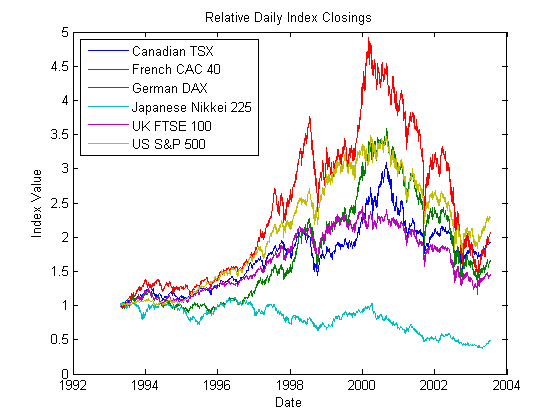
\includegraphics[width=\textwidth]{Line_Plot_2D_2_01.png}
                \caption{Stock Indices\cite{matlab_gallery} }
        \end{subfigure}%
        ~
        \begin{subfigure}[b]{0.4\textwidth}
                \centering
                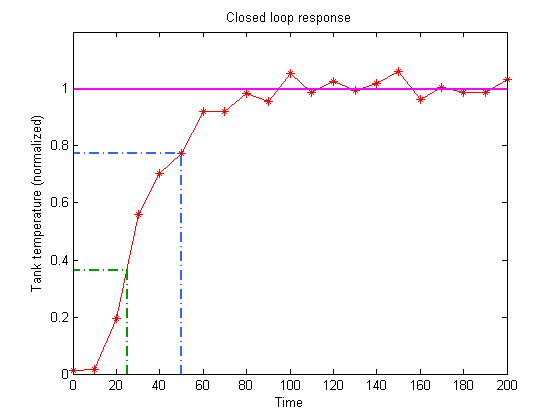
\includegraphics[width=\textwidth]{Add_Lines_to_Plot_1_01.png}
                \caption{Step Response\cite{matlab_gallery}}
        \end{subfigure}
\end{figure}

  
\end{frame}
%=========================================================================================
\begin{frame}[fragile]
\frametitle{Basic Line Plot}

\begin{block}{Syntax}
\begin{itemize}[<+->]
    \item To create an empty figure, call
          \begin{matlabcodebeamer}[frame=none]
          figure;
          \end{matlabcodebeamer}
    \item To create a line plot of vector \texttt{x} versus vector \texttt{t}, use
          \begin{matlabcodebeamer}[frame=none]
          plot(t,x);
          \end{matlabcodebeamer}
    \item You can input more vector pairs like
          \begin{matlabcodebeamer}[frame=none]
          plot(t1,x1,t2,x2);
          \end{matlabcodebeamer}
\end{itemize}
\end{block}
\end{frame}
%=========================================================================================
\begin{frame}[fragile]
\frametitle{Basic Line Plot}

\begin{block}{Syntax}
\begin{itemize}[<+->]
    \item Adding labels on axis 
          \begin{matlabcodebeamer}[frame=none]
          xlabel('x label');
          ylabel('y label');
          \end{matlabcodebeamer}
    \item Add title
          \begin{matlabcodebeamer}[frame=none]
          title('title for the figure');
          \end{matlabcodebeamer}
    \item Turn on/off the grid lines
          \begin{matlabcodebeamer}[frame=none]
          grid on;
          grid off;
          \end{matlabcodebeamer}
    \item Adding legends
          \begin{matlabcodebeamer}[frame=none]
          legend('first','second',...);
          \end{matlabcodebeamer}
\end{itemize}
\end{block}
\end{frame}
%=========================================================================================
\begin{frame}[fragile]
\frametitle{Basic Line Plot}
\textbf{Exercise} 
Visualizing $\sin(t)$ and $\cos(t)$ on $0 \leq t \leq 2\pi$. \pause
\begin{figure}[htb]
        \centering
        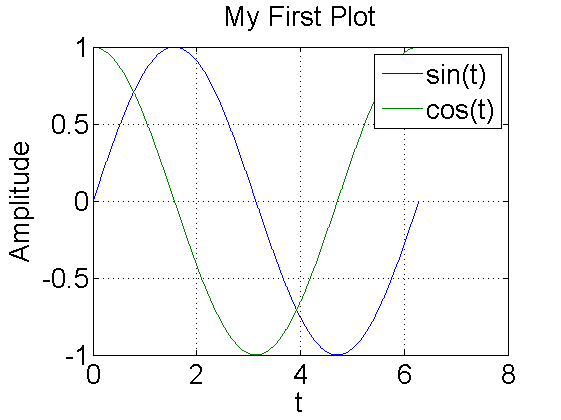
\includegraphics[width=6cm]{basic_plot_sine.eps}
\end{figure}

\end{frame}
%=========================================================================================
\begin{frame}[fragile]
\frametitle{Line Style}

\begin{itemize}[<+->]
    \item Using the \textit{string specifier} to change the line style.
    \item The \textit{string specifiers} contains
          \begin{itemize}
          \item Line style: \texttt{\{'-','--',':','-.','none'\}}
          \item Marker symbol: \texttt{\{'+','o','*','.','x'\}} and more.
          \item Color: \texttt{\{'r','g','b','w','k'\}}.
          \end{itemize}
    \item For example,
          \begin{matlabcode}[numbers=none,frame=none]
          plot(t,x,'--or');
          plot(t,x,'r',t,y,'-.xk');
          \end{matlabcode}

%    \item RGB triple is a 3-vector
%          \begin{matlabcode}[numbers=none,frame=none]
%          c = [r b g];
%          \end{matlabcode}
%          where \texttt{r,g,b} are real numbers between 0 and 1.
%    \item Color picker: returns a RGB triple
%          \begin{matlabcode}[numbers=none,frame=none]
%          c = uisetcolor;
%          \end{matlabcode}
\end{itemize}

\end{frame}
%=========================================================================================
\begin{frame}{Line Style}
\textbf{Exercise}
Let
\begin{equation}
    x(t) = t^2 \cos(5t) \e^{-t}.
\end{equation}\pause
The envelope of $x(t)$ is
\begin{equation}
    y(t) = \pm t^2 \e^{-t}.
\end{equation}\pause

Please duplicate the figure shown below:
\begin{figure}[htb]
        \centering
        \includegraphics[width=5cm]{ex_line_style.eps}
\end{figure}

\end{frame}
%=========================================================================================
\begin{frame}[fragile]
\frametitle{Plotting Complex Data}

\begin{block}{Syntax}
\begin{itemize}[<+->]
    \item To plot complex array \texttt{x}, use
          \begin{matlabcodebeamer}[frame=none]
          plot(x);
          \end{matlabcodebeamer}
    \item It is equivalent to
          \begin{matlabcodebeamer}[frame=none]
          plot(real(x),imag(x));
          \end{matlabcodebeamer}
\end{itemize}
\end{block}

\end{frame}
%=========================================================================================
\begin{frame}[fragile]
\frametitle{Plotting Complex Data}
\textbf{Example} 
Visualizing the distribution of the eigenvalues of the random matrix. \pause
\begin{itemize}
    \item Let \texttt{H} be an $n$-by-$n$ random matrix.
    \item Let \texttt{x} be its eigenvalues.
\end{itemize}

\pause
\begin{figure}[htb]
        \centering
        \includegraphics[width=5cm]{random_matrix_eigenvalue.eps}
\end{figure}

\end{frame}
%=========================================================================================
\begin{frame}[fragile]
\frametitle{Plotting Matrix Data}

\begin{block}{Syntax}
\begin{itemize}[<+->]
    \item By default \tttbf{plot}\texttt{(Y)} will plot each column of \texttt{Y}.
    \item When specifying the \texttt{x} vector,
          \begin{matlabcodebeamer}[frame=none]
          plot(x,Y);
          \end{matlabcodebeamer}
          will try to match the dimension of \texttt{x} and \texttt{Y}.
\end{itemize}
\end{block}

\end{frame}
%=========================================================================================
\begin{frame}[fragile]
\frametitle{Plotting Matrix Data}
\textbf{Example} 
Plot \texttt{y = randn(5,3)} with and without \texttt{x = 1:3}.\pause
\setcounter{subfigure}{0}
\begin{figure}
        \begin{subfigure}[b]{0.3\textwidth}
                \centering
                \includegraphics[width=\textwidth]{plot_matrix_data1.eps}
                \caption{Without \texttt{x}.}
        \end{subfigure}%
        ~\pause
        \begin{subfigure}[b]{0.3\textwidth}
                \centering
                \includegraphics[width=\textwidth]{plot_matrix_data2.eps}
                \caption{With \texttt{x}.}
        \end{subfigure}
\end{figure}

\end{frame}
%=========================================================================================
\begin{frame}[fragile]
\frametitle{Plotting Multiple Lines On the Same Axes}
\begin{itemize}[<+->]
    \item If you call \tttbf{plot} twice, the first plot will be erased.
    
    \item To retain current graph when adding new graph, tell Matlab to
          \begin{matlabcode}[frame=none]
          hold on;
          \end{matlabcode}
          
    \item If you want different lines to have different color, use
          \begin{matlabcode}[frame=none]
          hold all;
          \end{matlabcode}
          
    \item The default is
          \begin{matlabcode}[frame=none]
          hold off;
          \end{matlabcode}
\end{itemize}

\end{frame}
%=========================================================================================
\begin{frame}[fragile]
\frametitle{Plotting Multiple Lines On the Same Axes}
\textbf{Exercise}
In our first sine wave example, we use
\begin{matlabcode}[frame=none]
          plot(t,x,t,y)
\end{matlabcode}\pause
          
Now try
\begin{matlabcode}[frame=none]
          plot(t,x);
          hold all;
          plot(t,y);
\end{matlabcode}

Change \texttt{'all'} to \texttt{'on'} and \texttt{'off'}.

\end{frame}
%=========================================================================================
\begin{frame}{Hierarchy of The Graphic Objects}
A Matlab plot is composed of (at least) three objects:
\setcounter{subfigure}{0}
\begin{figure}
        \begin{subfigure}[b]{0.3\textwidth}
                \centering
                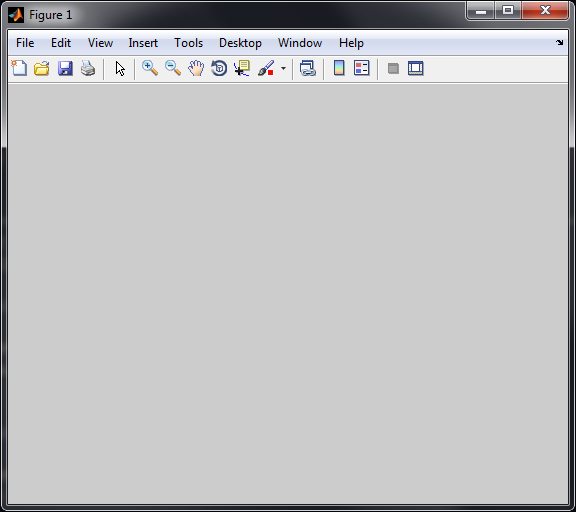
\includegraphics[width=\textwidth]{figure_window.png}
                \caption{Figure window.}
        \end{subfigure}%
        ~\pause
        \begin{subfigure}[b]{0.3\textwidth}
                \centering
                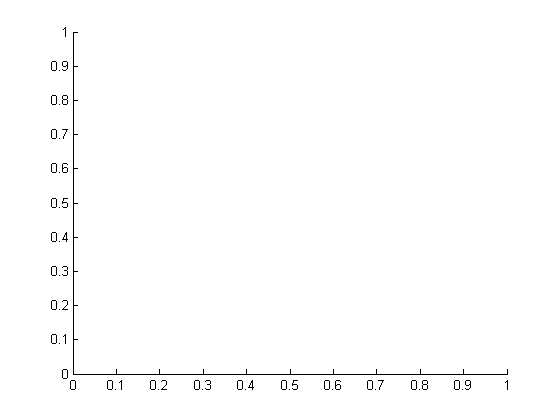
\includegraphics[width=\textwidth]{empty_axis.png}
                \caption{Axis object.}
        \end{subfigure}
        ~\pause
        \begin{subfigure}[b]{0.3\textwidth}
                \centering
                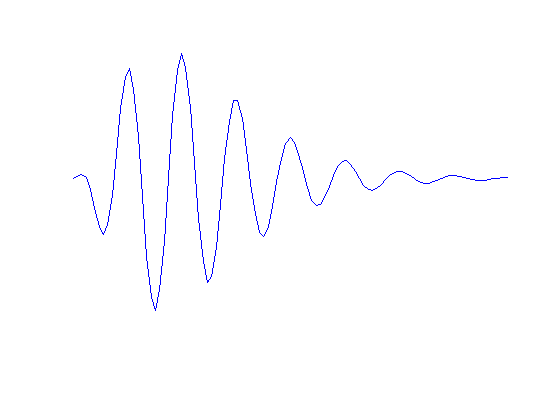
\includegraphics[width=\textwidth]{lineseries_object.png}
                \caption{Line series object.}
        \end{subfigure}
\end{figure}

\end{frame}
%=========================================================================================
\begin{frame}[fragile]
\frametitle{Hierarchy of The Graphic Objects}
\begin{itemize}[<+->]
    \item Each object has a unique identifier, called the \textbf{handle}.
    
    \item You can ask Matlab to get and set the properties of the object with its handle.
    
    \item To get the handle of the current figure, type
          \begin{matlabcode}[frame=none]
          h_fig = gcf;
          \end{matlabcode}
          
    \item To get the handle of the current axis, type
          \begin{matlabcode}[frame=none]
          h_ax = gca;
          \end{matlabcode}
          
    \item To get the handle of the line series, use
          \begin{matlabcode}[frame=none]
          h = plot(t,x);
          \end{matlabcode}
\end{itemize}

\end{frame}
%=========================================================================================
\begin{frame}[fragile]
\frametitle{Set and Get}
\begin{itemize}
    \item Get the value of the property:
          \begin{matlabcode}[frame=none]
          value = get(h,'PropertyName');
          \end{matlabcode}
          
    \item Set using property-value pair:
          \begin{matlabcode}[frame=none]
          set(h,'PropertyName',value);
          \end{matlabcode}
\end{itemize}
Complicated? Let's try an example.
\end{frame}
%=========================================================================================
\begin{frame}[fragile]
\frametitle{Set and Get}
\textbf{Example} 
Plot $\sin(t)$ and $\cos(t)$. Change the line width and fine-tune the axis.
\setcounter{subfigure}{0}
\begin{figure}
    \centering
    \includegraphics[width=6cm]{set_axis_lineseries.eps}
\end{figure}

\end{frame}
%=========================================================================================
\begin{frame}[fragile]
\frametitle{Linear and Log Scale}
\begin{itemize}[<+->]
    \item By default \tttbf{plot} use linear scale on both axis.
    
    \item Replace \tttbf{plot} by
    \begin{itemize}
        \item \tttbf{semilogx}
        \item \tttbf{semilogy}
        \item \tttbf{loglog}
    \end{itemize}        
    
    \item Equivalently, use 
          \begin{matlabcode}[numbers=none,frame=none]
          set(gca, 'XScale', 'log');
          \end{matlabcode}
          and/or
          \begin{matlabcode}[numbers=none,frame=none]
          set(gca, 'YScale', 'log');
          \end{matlabcode}
\end{itemize}

\end{frame}
%=========================================================================================
\begin{frame}[fragile]
\frametitle{Linear and Log Scale}
\textbf{Example} 
The transfer function of a second order system has the form
$$H(s) = \frac{\omega_n^2}{s^2 + 2 \zeta \omega_n s + \omega_n^2},$$
where $\zeta$ is the damping ratio and $\omega_n$ is the natural frequency.
\pause
The frequecny response of a system is characterized by
\begin{itemize}
    \item The magnitude $|H(\jmath \omega)|$
    \item The phase $\angle H(\jmath \omega)$
\end{itemize}

In this example, we will plot the frequency response of $H(s)$.

\end{frame}
%=========================================================================================
\begin{frame}[fragile]
\frametitle{Linear and Log Scale}

\setcounter{subfigure}{0}
\begin{figure}
    \centering
    \includegraphics[width=6cm]{log_scale.eps}
    \caption{Frequency response of $H(s)$.}
\end{figure}

\end{frame}
%=========================================================================================
\begin{frame}[fragile]
\frametitle{Subplot}

\begin{block}{Syntax}
          \begin{matlabcodebeamer}[frame=none]
          subplot(m,n,1);
          plot(t,x);
          \end{matlabcodebeamer}
Will create a $m$-by-$n$ subplot and place the plot of \texttt{x} versus \texttt{t} at location 1.
\end{block}
\end{frame}
%=========================================================================================
\begin{frame}[fragile]
\frametitle{Subplot}
\textbf{Example} 
Create 25 subplots of sine wave with increasing frequency.
\setcounter{subfigure}{0}
\begin{figure}
    \centering
    \includegraphics[width=6cm]{subplot_sine.eps}
\end{figure}

\end{frame}
%=========================================================================================
\section{GUI and More 2D Plots}
\begin{frame}[fragile]
\frametitle{Adding Annotations}

\begin{block}{Syntax}

If you want to put \texttt{'some text'} at location \texttt{(x,y)}, type
\begin{matlabcodebeamer}[numbers=none,frame=none]
          text(x,y,'some text');
\end{matlabcodebeamer}
\end{block}

\end{frame}
%=========================================================================================
\begin{frame}[fragile]
\frametitle{Adding Annotations}
\textbf{Example} 

\setcounter{subfigure}{0}
\begin{figure}
    \centering
    \includegraphics[width=6cm]{set_axis_lineseries_text.eps}
\end{figure}

\end{frame}
%=========================================================================================
\begin{frame}[fragile]
\frametitle{Adding Annotations}
\begin{itemize}[<+->]
    \item It's a pain to calculate the coordinates, is there any easier way?
    
    \item Luckily, Matlab provides a useful function
          \begin{matlabcode}[numbers=none,frame=none]
          gtext('some text');
          \end{matlabcode}

    \item Click on the figure to place the text.
\end{itemize}

\end{frame}
%=========================================================================================
\begin{frame}[fragile]
\frametitle{GUI}
It's about time to talk about the Graphical User Interface (GUI).

Pros:
\begin{itemize}
    \item Easy to use.
    \item No need to remember many commands.
\end{itemize}
\pause
Cons:
\begin{itemize}
    \item Less flexible.
    \item Can not batch process.
\end{itemize}
\pause
\begin{block}{Go with GUI if}
\begin{itemize}
    \item There are only a few figures to edit.
    \item No need to edit them in the future.
\end{itemize}

Otherwise using commands will be more efficient.
\end{block}
\end{frame}
%=========================================================================================
\begin{frame}[fragile]
\frametitle{Saving and Exporting}
Some tips about exporting figures:
\begin{itemize}[<+->]
    \item Try to save to vector format.
    \item Use `copy figure' on Windows.
    \item Keep a \texttt{.fig} copy so you can edit it later.
\end{itemize}

\end{frame}
%=========================================================================================
\begin{frame}[fragile]
\frametitle{Histogram}

\begin{block}{Syntax}
\begin{itemize}[<+->]
    \item Create a histogram of data vector \texttt{x}
          \begin{matlabcodebeamer}[numbers=none,frame=none]
          hist(x);
          \end{matlabcodebeamer}
%    \item To specify number of bins, use
%          \begin{matlabcodebeamer}[numbers=none,frame=none]
%          hist(x,m);
%          \end{matlabcodebeamer}
\end{itemize}
\end{block}

\end{frame}
%=========================================================================================
\begin{frame}[fragile]
\frametitle{Histogram}
\textbf{Example} 
Linear Congruential Generator (LCG)

\begin{itemize}[<+->]
    \item LCG is a popular (and old) Pseudo-Random Numbers Generator.
    \item Simple and efficient to compute.
    \item Well understood.
    \item Poor choice of parameters lead to bad performance.
\end{itemize}
\pause
\begin{block}{LCG}
\begin{equation}
    x_{n+1} \equiv \left( a x_n + b \right)~~\pmod{m},
\end{equation}
\begin{itemize}
    \item $m > 0$: the modulus
    \item $a > 0$: the multiplier
    \item $b \geq 0$: the increment
    \item $x_0$: the seed
\end{itemize}
\end{block}

\end{frame}
%=========================================================================================
\begin{frame}[fragile]
\frametitle{Histogram}
\textbf{Exercise} 
Use
\begin{itemize}
    \item $a = 3$
    \item $b = 0$
    \item $m = 31$
    \item $x_0 = 1$
\end{itemize}
Generate $100$ samples to find its distribution.
\setcounter{subfigure}{0}
\begin{figure}
    \centering
    \includegraphics[width=5cm]{lcg_histogram.eps}
\end{figure}

\end{frame}
%=========================================================================================
\begin{frame}[fragile]
\frametitle{Bar Chart}

\begin{block}{Syntax}
\begin{itemize}[<+->]
    \item Create a bar chart
          \begin{matlabcodebeamer}[numbers=none,frame=none]
          bar(Y);
          \end{matlabcodebeamer}
          Each column of \texttt{Y} will have the same color and rows are grouped together.
    \item It is equivalent to
          \begin{matlabcodebeamer}[numbers=none,frame=none]
          bar(Y,'grouped');
          \end{matlabcodebeamer}
          Try \texttt{'stacked'} instead of \texttt{'grouped'}.
\end{itemize}
\end{block}

\end{frame}
%=========================================================================================
\begin{frame}[fragile]
\frametitle{Bar Chart}
\textbf{Example} 

\setcounter{subfigure}{0}
\begin{figure}
    \centering
    \includegraphics[width=6cm]{bar_chart.eps}
\end{figure}

\end{frame}
%=========================================================================================
\begin{frame}[fragile]
\frametitle{Area Plot}

\begin{block}{Syntax}
\begin{itemize}
    \item Stacks each data series and fill the underlying area with different colors
          \begin{matlabcodebeamer}[numbers=none,frame=none]
          area(X,Y);
          \end{matlabcodebeamer}
\end{itemize}
\end{block}

\end{frame}
%=========================================================================================
\begin{frame}[fragile]
\frametitle{Area Plot}
\textbf{Example} 

\setcounter{subfigure}{0}
\begin{figure}
    \centering
    \includegraphics[width=6cm]{area_plot.eps}
\end{figure}

\end{frame}
%=========================================================================================
\begin{frame}[fragile]
\frametitle{Stem Plot}
Stem plot is useful for visualizing discrete time data.

\begin{block}{Syntax}
\begin{itemize}
    \item Use exactly like the \tttbf{plot} function
          \begin{matlabcodebeamer}[numbers=none,frame=none]
          stem(t,x);
          \end{matlabcodebeamer}
\end{itemize}
\end{block}

\end{frame}
%=========================================================================================
\begin{frame}[fragile]
\frametitle{Stem Plot}
\textbf{Example} 

\setcounter{subfigure}{0}
\begin{figure}
    \centering
    \includegraphics[width=6cm]{stem_sine.eps}
\end{figure}

\end{frame}
%=========================================================================================
\begin{frame}[fragile]
\frametitle{Polar Plot}
\begin{itemize}[<+->]
    \item Sometimes it is easier to express coordinate in the polar form.
    \item Let $(x,y)$ be the coordinates in the Cartesian coordinate system, its corresponding polar coordinates is given by
\begin{align}
    r      &= \sqrt{x^2 + y^2} \\
    \theta &= \tan^{-1}(y/x).
\end{align}
\end{itemize}

\pause
\begin{block}{Syntax}
\begin{itemize}
    \item Plot \texttt{r} versus \texttt{theta} in the polar coordinate
          \begin{matlabcodebeamer}[numbers=none,frame=none]
          polar(theta,r);
          \end{matlabcodebeamer}
\end{itemize}
\end{block}

\end{frame}
%=========================================================================================
\begin{frame}[fragile]
\frametitle{Polar Plot}
\textbf{Example} 
The butterfly fly curve, discovered by Temple H. Fay, is generated by the equations
\begin{equation}
r=e^{\sin \theta} - 2 \cos (4 \theta ) + \sin^5\left(\frac{2 \theta - \pi}{24}\right).
\end{equation}\pause

\setcounter{subfigure}{0}
\begin{figure}
    \centering
    \includegraphics[width=5cm]{polar_butterfly_curve.eps}
\end{figure}

\end{frame}
%=========================================================================================
\begin{frame}[fragile]
\frametitle{Scatter Plot}
Scatter plot is used to visualize the distribution of two dimensional data.

\begin{block}{Syntax}
\begin{itemize}
    \item to generate the scatter plot for the data vector \texttt{X} and \texttt{Y}
          \begin{matlabcodebeamer}[numbers=none,frame=none,backgroundcolor=\color{blockbody}]
          scatter(X,Y)
          \end{matlabcodebeamer}
\end{itemize}
\end{block}


\end{frame}
%=========================================================================================
\begin{frame}[fragile]
\frametitle{Scatter Plot}
\textbf{Example} Linear Fitting

\begin{itemize}[<+->]
    \item Suppose we are given a data set \texttt{x} and \texttt{y}.
    \item It is assumed that $y = ax + b + \mbox{noise}$.
    \item Find the best linear fit $\hat{y} = \hat{a} x + \hat{b}$.
\end{itemize}
\pause
\setcounter{subfigure}{0}
\begin{figure}
    \centering
    \includegraphics[width=6cm]{scatter_linear_fitting.eps}
\end{figure}

\end{frame}
%=========================================================================================
\begin{frame}[fragile]
\frametitle{Contour Plot}

\begin{block}{Syntax}
\begin{itemize}[<+->]
    \item The basic syntax is
          \begin{matlabcodebeamer}[numbers=none,frame=none]
          contour(Z);
          \end{matlabcodebeamer}
    \item You can specify the number of contour level
          \begin{matlabcodebeamer}[numbers=none,frame=none]
          contour(Z, n_level);
          \end{matlabcodebeamer}
\end{itemize}
\end{block}
\end{frame}
%=========================================================================================
\begin{frame}[fragile]
\frametitle{Contour Plot}
\textbf{Example} Visualizing \texttt{peaks}

The Matlab function \texttt{peaks} is defined as
\begin{equation}
    z = 3(1-x)^2 \e^{-x^2 - (y+1)^2} - 10(\frac{x}{5}-x^3-y^5)\e^{-x^2-y^2}-
    \frac{1}{3}\e^{-(x+1)^2-y^2}.
\end{equation}\pause

\setcounter{subfigure}{0}
\begin{figure}
    \centering
    \includegraphics[width=6cm]{contour_peaks.eps}
\end{figure}

\end{frame}
%=========================================================================================
\begin{frame}[fragile]
\frametitle{Animation}
The simplest way to generate animation in Matlab is use the template
\begin{matlabcode}[numbers=none,frame=none]
          figure;
          % Prevent Matlab reseting your view angle.
          hold on;    
          for I=1:N
              % Update your data here.
              plot(t,x);  % Draw new frame.
              pause(0.1); % Pause for 0.1 seconds.
          end
\end{matlabcode}

\end{frame}
%=========================================================================================
\section{3D Plots}
\begin{frame}[fragile]
\frametitle{3D Plot}
\begin{figure}
        \begin{subfigure}[b]{0.4\textwidth}
                \centering
                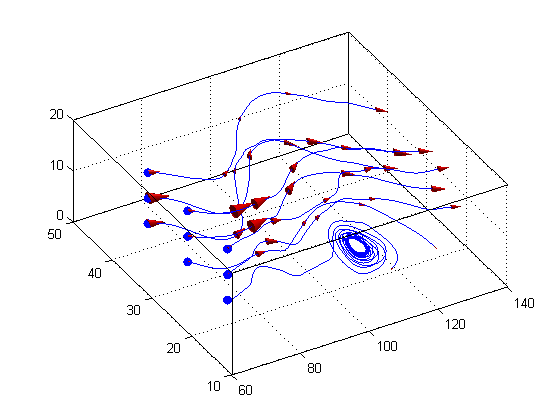
\includegraphics[width=\textwidth]{Streamline_01.png}
                \caption{Stream lines\cite{matlab_gallery} }
        \end{subfigure}%
        ~
        \begin{subfigure}[b]{0.4\textwidth}
                \centering
                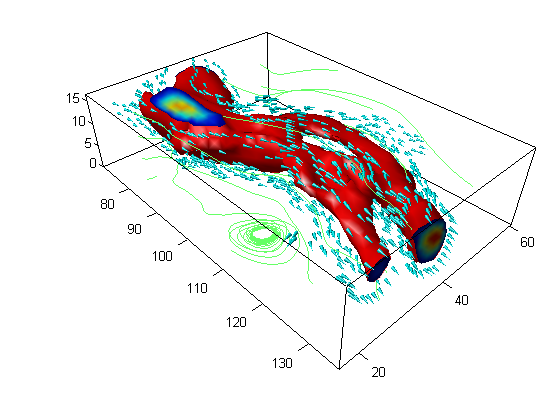
\includegraphics[width=\textwidth]{Wind_01.png}
                \caption{Wind Field\cite{matlab_gallery}}
        \end{subfigure}
\end{figure}

\end{frame}
%=========================================================================================
\begin{frame}[fragile]
\frametitle{3D Line Plot}
\begin{block}{Syntax}
\begin{itemize}
    \item Plot lines in 3D
          \begin{matlabcodebeamer}[numbers=none,frame=none]
          plot3(x,y,z);
          \end{matlabcodebeamer}
\end{itemize}
\end{block}

\end{frame}
%=========================================================================================
\begin{frame}[fragile]
\frametitle{3D Line Plot}
\textbf{Example} 3D Brownian Motion:
the position $\vx_n$ of a Brownian particle at time $n$ is given by
\begin{equation}
    \vx_n = \vx_{n-1} + \vv,
\end{equation}
where $\vv$ is a standard normal random vector.

\setcounter{subfigure}{0}
\begin{figure}
    \centering
    \includegraphics[width=6cm]{plot3D_brownian_motion.eps}
\end{figure}

\end{frame}
%=========================================================================================
\begin{frame}[fragile]
\frametitle{3D Line Plot}
\textbf{Example} Lorenz Attractor

Lorenz system is a simplified model for atmospheric convection, it is modeled by the ordinary differential equations
 \begin{align}
\frac{dx}{dt} &= \sigma (y - x), \\
\frac{dy}{dt} &= x (\rho - z) - y, \\
\frac{dz}{dt} &= x y - \beta z,
\end{align} 
where $x$, $y$ and $z$ are the coordinate of the state, $t$ represents time, $\rho$, $\sigma$ and $\beta$ are parameters.


\end{frame}
%=========================================================================================
\begin{frame}[fragile]
\frametitle{3D Line Plot}
\textbf{Example} Lorenz Attractor

\setcounter{subfigure}{0}
\begin{figure}
    \centering
    \includegraphics[width=6cm]{lorenz_attractor.eps}
\end{figure}

\end{frame}
%=========================================================================================
\begin{frame}[fragile]
\frametitle{Mesh Plot}
Mesh plot is used to visualize 2D scalar fields.
\begin{block}{Syntax}
\begin{itemize}
    \item Plot \texttt{Z} as a function of \texttt{X} and \texttt{Y}
          \begin{matlabcodebeamer}[numbers=none,frame=none]
          mesh(X,Y,Z);
          \end{matlabcodebeamer}
\end{itemize}
\end{block}

\end{frame}
%=========================================================================================
\begin{frame}[fragile]
\frametitle{Mesh Plot}
\textbf{Example} 3D Sinc function

The 3D sinc function is defined as
\begin{equation}
    \sinc(\vx) = \frac{\sin(\| \vx \|)}{\| \vx \|}.
\end{equation}\pause

\setcounter{subfigure}{0}
\begin{figure}
    \centering
    \includegraphics[width=6cm]{mesh_3D_sinc.eps}
\end{figure}

\end{frame}
%=========================================================================================
\begin{frame}[fragile]
\frametitle{Surface Plot}
Surface plot is mesh plot plus patches.
\begin{block}{Syntax}
\begin{itemize}
    \item Plot \texttt{Z} as a function of \texttt{X} and \texttt{Y}
          \begin{matlabcodebeamer}[numbers=none,frame=none]
          surf(X,Y,Z);
          \end{matlabcodebeamer}
\end{itemize}
\end{block}

\end{frame}
%=========================================================================================
\begin{frame}[fragile]
\frametitle{Surface Plot}
\textbf{Example} 3D Sinc function

\setcounter{subfigure}{0}
\begin{figure}
    \centering
    \includegraphics[width=6cm]{surf_3D_sinc.eps}
\end{figure}

\end{frame}
%=========================================================================================
\begin{frame}[fragile]
\frametitle{Surface Plot}
\textbf{Example} 2D Wave Equation

The wave equation is a partial differential equation
\begin{equation}\label{eq:wave_eq}
   u_{tt} = c^2 \Delta u - b u_t,\quad \mbox{where}
\end{equation}\pause
\begin{itemize}
    \item $c$ is the wave speed
    \item $b$ is the damping coefficient
    \item $\Delta$ is Laplacian, defined as
          \begin{equation}
          \Delta u = u_{xx} + u_{yy}.
          \end{equation}
\end{itemize}
\pause
We use the Finite Difference Method (FDM) to approximate
\begin{equation}
    u_t \approx \frac{u(t+dt) - u(t)}{dt}.
\end{equation}

\end{frame}
%=========================================================================================
\begin{frame}[fragile]
\frametitle{Surface Plot}
\textbf{Example} 2D Wave Equation

\setcounter{subfigure}{0}
\begin{figure}
    \centering
    \includegraphics[width=6cm]{wave_fdm.eps}
\end{figure}

\end{frame}
%=========================================================================================
\begin{frame}[fragile]
\frametitle{2D Vector Field}
\begin{block}{Syntax}
\begin{itemize}
    \item Plot the vector field \texttt{Zx} and \texttt{Zy} as a function of \texttt{X} and \texttt{Y}
          \begin{matlabcodebeamer}[numbers=none,frame=none]
          quiver(X,Y,Zx,Zy);
          \end{matlabcodebeamer}
\end{itemize}
\end{block}

\end{frame}
%=========================================================================================
\begin{frame}[fragile]
\frametitle{2D Vector Field}
\textbf{Example} Gradient of Scalar Field

The easiest way to generate a vector field is to find the gradient of some scalar field $f$
\begin{equation}
    \nabla f = \frac{\partial}{\partial x} f \ve_x + \frac{\partial}{\partial y} f \ve_y 
\end{equation}
\pause
Try
\begin{equation}
    f(x) = x^2 - 3\sin(xy).
\end{equation}

\begin{figure}
    \centering
    \includegraphics[width=5cm]{quiver_gradient.eps}
\end{figure}

\end{frame}
%=========================================================================================
\begin{frame}[allowframebreaks]
\frametitle{Reference}
  \begin{thebibliography}{10}    
  \bibitem{matlab_gallery}
    MathWorks
    \newblock {MATLAB Plot Gallery}.
    \newblock MATLAB Plot Gallery, 2012. MathWorks, Inc. 10 Sep. 2012
  \end{thebibliography}

  \begin{thebibliography}{10}    
  \bibitem{matlab_doc}
    MathWorks
    \newblock {MATLAB Documentation}.
    \newblock MATLAB Documentation, 2012. MathWorks, Inc. 10 Sep. 2012
  \end{thebibliography}

  \begin{thebibliography}{10}    
  \bibitem{matlab_handle}
    Green, R.A. 
    \newblock {Getting a handle on Matlab graphics}.
    \newblock IEEE Potentials, 2007. Volume: 26 , Issue: 4 
  \end{thebibliography}
  
  \begin{thebibliography}{10}    
  \bibitem{moler}
    Moler, Cleve
    \newblock {Numerical Computing with MATLAB}.
    \newblock Textbooks by Cleve Moler, 2004. MathWorks, Inc. 10 Sep. 2012
  \end{thebibliography}
  
\end{frame}







\end{document}
%%% Local Variables:
%%% mode: latex
%%% TeX-master: t
%%% End:
